\documentclass{article}
\usepackage{pdflscape}
\usepackage[margin=1in]{geometry}
\usepackage{verbatim}
\usepackage{graphicx, float}
\author{Astrid Augusta Yu}
\title{CPE 233 Lab \#2 -- Program Counter}
\date{\today}

\usepackage{amsmath}
\usepackage{amsfonts}
\usepackage{amssymb}
\DeclareMathOperator\bit{bit}
\DeclareMathOperator\byte{byte}
\DeclareMathOperator\word{word}
\DeclareMathOperator{\res}{RESET}
\DeclareMathOperator{\pcw}{PC\_WRITE}
\DeclareMathOperator{\pcs}{PC\_SOURCE}

\begin{document}
\maketitle

\section{HDL Code}

\subsection{pc\_mod.sv}

\begin{verbatim}
`timescale 1ns / 1ps
///////////////////////////////////////////////////////////////
// Company: Cal Poly
// Engineer: Astrid Yu
// 
// Create Date: 04/13/2020 02:05:38 PM
// Design Name: Program Counter Module
// Module Name: pc_mod
// Project Name: 
// Target Devices: 
// Tool Versions: 
// Description: Program Counter for the Otter MCU.
// 
// Dependencies: 
// 
// Revision:
// Revision 0.01 - File Created
// Additional Comments:
// 
///////////////////////////////////////////////////////////////


module pc_mod(
    input rst,
    input [31:0] jalr,
    input [31:0] jal,
    input [31:0] branch,
    input pc_write,
    input pc_source,
    input clk,
    output [13:0] addr
    );
    
    reg [13:0] data;
    assign addr = data;
    logic [13:0] next;
    
    always_comb begin
        case (pc_source) 
            2'd0: next = data + 1;
            2'd1: next = jalr[15:2];
            2'd2: next = branch[15:2];
            default: next = jal[15:2];
        endcase
    end
    
    always_ff @(posedge clk) begin
        if (rst)
            data <= 0;
        else if (pc_write) 
            data <= next;
    end
endmodule

    
\end{verbatim}

\subsection{top\_level.sv}

\begin{verbatim}
`timescale 1ns / 1ps
/////////////////////////////////////////////////////////////////
// Company: Cal Poly
// Engineer: Astrid Yu
// 
// Create Date: 04/13/2020 02:27:23 PM
// Design Name: Top Level
// Module Name: top_level
// Project Name: 
// Target Devices: 
// Tool Versions: 
// Description: A program counter connected to a RAM.
// 
// Dependencies: 
// 
// Revision:
// Revision 0.01 - File Created
// Additional Comments:
// 
/////////////////////////////////////////////////////////////////


module top_level(
    input rst,
    input pc_write,
    input [1:0] pc_source,
    input clk,
    output [31:0] ir
    );
    
    logic [13:0] addr;
    
    pc_mod pc(
        .*, 
        .jal(32'hCCCC), 
        .jalr(32'h4444), 
        .branch(32'h8888)
    );
    
    Memory memory(
        .MEM_CLK (clk),
        .MEM_RDEN1 (1),
        .MEM_RDEN2 (0),
        .MEM_WE2 (0),
        .MEM_ADDR1 (addr),
        .MEM_ADDR2 (0),
        .MEM_DIN2 (0),
        .MEM_SIZE (2),
        .MEM_SIGN (0),
        .IO_IN (0),
        .IO_WR (),
        .MEM_DOUT1 (ir),
        .MEM_DOUT2 ()
    );
        
endmodule

\end{verbatim}

\section{Assembly and Dump}

\subsection{Assembly}

\begin{verbatim}
.text
init:	li t0,41
        li t1,8
        li t2,12
main:   add t3,t2,t1
        sub t2,t2,t0
        sra t0,t2,t1
        j main
\end{verbatim}

\subsection{Dump}

\begin{verbatim}
00400293
00800313
00c00393
00638e33
405383b3
4063d2b3
ff5ff06f
\end{verbatim}

\section{Schematic}
\centering
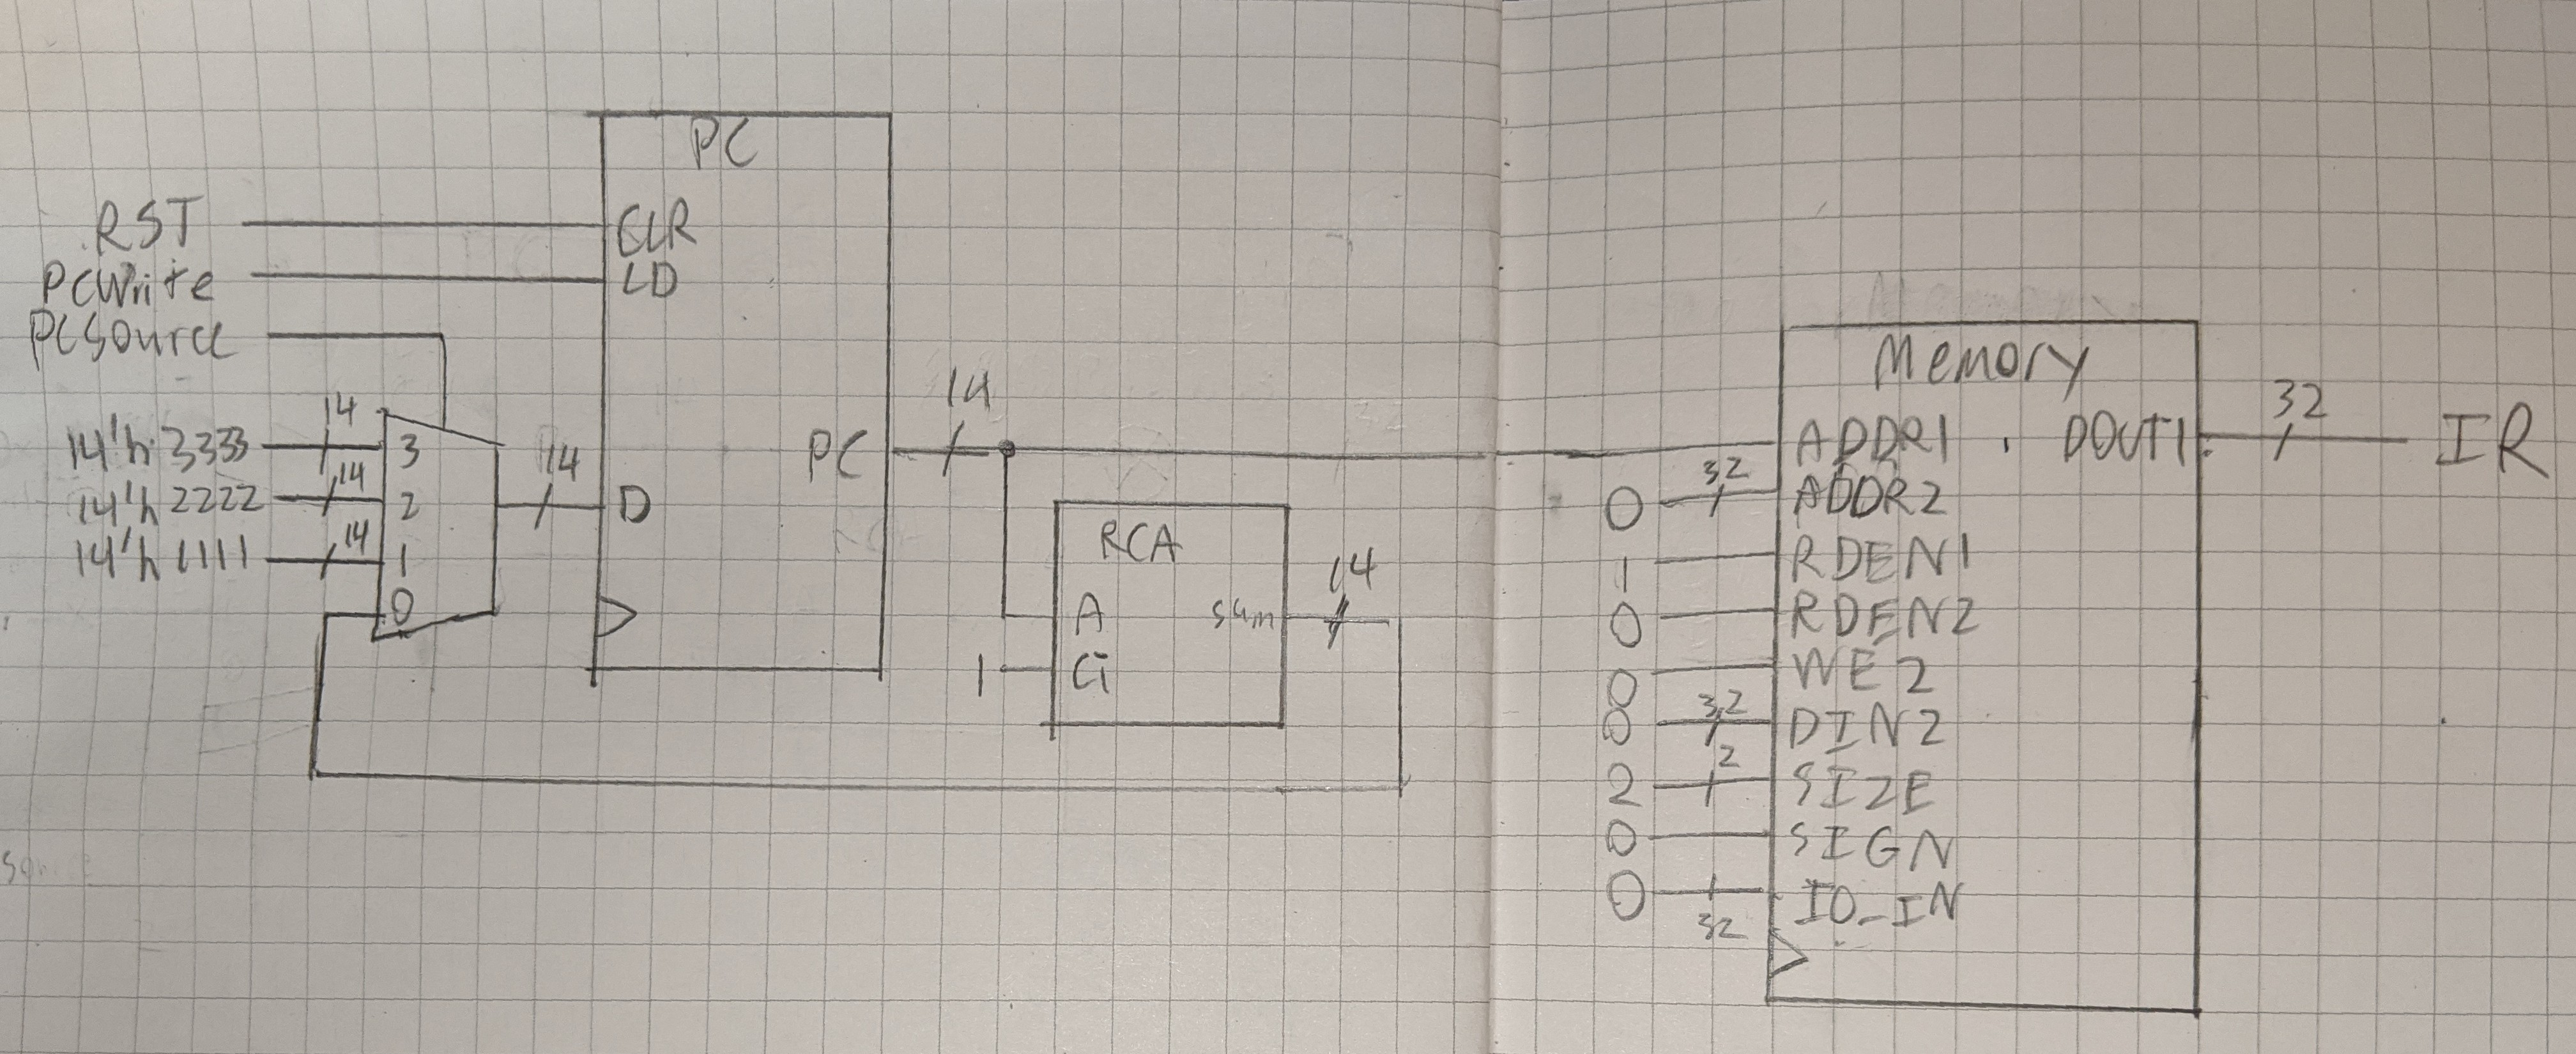
\includegraphics[width=\textwidth]{schem.jpg}

\begin{landscape}
    
\raggedright 
\section{Timing Diagrams}
\subsection{Overview}

\includegraphics[width=\linewidth]{woverview.png}

The full timing diagram. There are 4 distinct sections: the initial test, and 
3 nearly-identical sections for jalr, branch, and jal respectively. 

\subsection{Memory loaded correctly}
\includegraphics[width=\linewidth]{02.png}

ir matches exactly with the assembly dump above.

\subsection{Initial section}
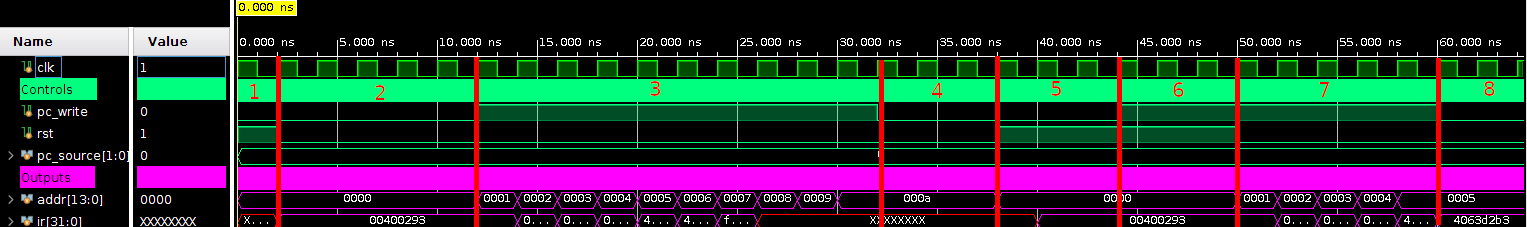
\includegraphics[width=\linewidth]{01.png}

\begin{enumerate}
    \item $\res\rightarrow$ addr = 0.
    \item $\overline{\res}, \overline{\pcw} \rightarrow$ addr does not increment even with $\pcs = 0$
    \item $\overline{\res}, \pcw , \pcs = 0\rightarrow$ addr increments.
    \item $\overline{\res}, \overline{\pcw} \rightarrow$ addr stops incrementing.
    \item $\res, \overline{\pcw} \rightarrow$ addr = 0
    \item $\res, \pcw \rightarrow$ addr = 0
    \item $\overline{\res}, \pcw , \pcs = 0\rightarrow$ addr increments again.
    \item $\overline{\res}, \overline{\pcw} \rightarrow$ addr stops incrementing.
\end{enumerate}

\subsection{Testing \texttt{jalr}}
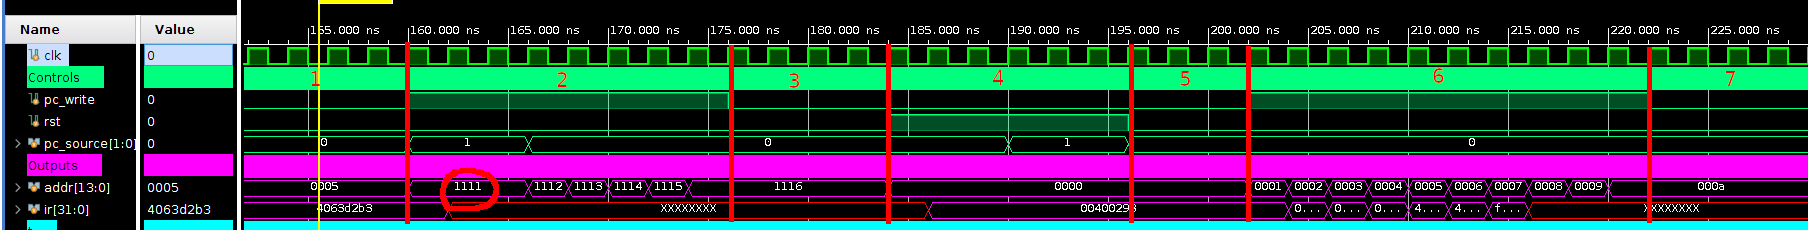
\includegraphics[width=\linewidth]{11.png}
\begin{enumerate}
    \item $\overline{\res}, \overline{\pcw} \rightarrow$ addr is frozen
    \item $\overline{\res}, \pcw, \pcs = 1 \rightarrow$ addr is set to 0x1111, as expected
    \item $\overline{\res}, \overline{\pcw} \rightarrow$ addr is frozen
    \item $\res, \overline{\pcw} \rightarrow$ addr set to 0. Still at 0 even when $\pcs = 1$
    \item $\overline{\res}, \overline{\pcw} \rightarrow$ addr is frozen
    \item $\overline{\res}, \pcw, \pcs = 0\rightarrow$ addr increments
    \item $\overline{\res}, \overline{\pcw} \rightarrow$ addr is frozen
\end{enumerate}

\subsection{Testing \texttt{branch}}
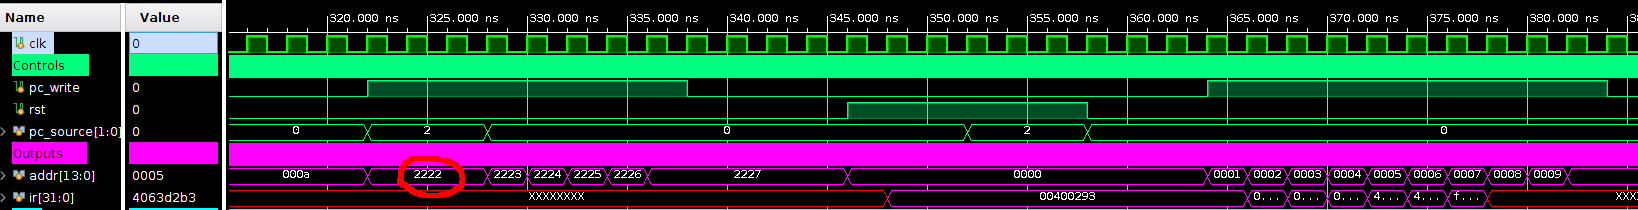
\includegraphics[width=\linewidth]{20.png}

$\pcs = 2 \rightarrow$ addr set to 0x2222

Otherwise, same behavior as \texttt{jalr}

\subsection{Testing \texttt{jal}}
\includegraphics[width=\linewidth]{30.png}

$\pcs = 2 \rightarrow$ addr set to 0x2222

Otherwise, same behavior as \texttt{jalr}

\end{landscape}

\raggedright
\section{Questions}

\begin{enumerate}
    \item The PC needs to be a register instead of a counter because it needs to be able to perform jumps and such.
    \item clk, PCWrite, pcSource, and rst are control signals. jalr, branch, and jal are data signals.
    \item The RAM's output always lags behind the address input by 1 clock cycle. Therefore, if the program counter
        advanced every clock cycle, it would never output the memory at the location associated with the program counter's
        address.
    \item They are not attached to the memory because the PC jumps 4 words at a time. Those values are guaranteed to be
        zero due to this property.
    \item jal will always jump to the same location, but jalr reads the location to jump to from the register.
        Because of this difference, jal would be sourced from the memory and jalr would be sourced from
        a register.
    \item The memory has 16384 32-bit words. Therefore, the memory capacity is 16384 words, or $16384 \word \times \frac{32 \bit}{\word} \times \frac{\byte}{8 \bit} = 16384 \byte$
    \item The assembler may not be deterministic; i.e. it might not output the same machine code every time it is compiled.
    \item The .mem file only filled up addresses 0x00000000 through 0x00000006. jal, jalr, and branch were all outside
        of that address space, so they were looking at data that was not initialized.
    \item The PC advanced by 4 every time because the MCU's instructions are all $32 \bit = 8 \byte$s wide.
    \item There is no need for an IOBUS\_OUT port. The microcontroller-out, peripheral-in function can be easily done with 
    the MEM\_DOUT port. 
\end{enumerate}

\section{Programming Assignment}

\subsection{Part 1}

\begin{verbatim}
;----------------------------------------------------------------
;- Reads data from the input port addressed by 0xC000_0012, 
;- multiplies that data by three, then outputs data to the 
;- output port addressed by 0xC000_0033.
;-
;- Tweaked registers: t0, t1
;----------------------------------------------------------------
.text
load:
	# Load the memory at 0xC000_0012 into t0
	li t0, 0xc0000012
	lw t1, 0(t0)

calc:
    # Multiply t0 by 3 and store in t1
    slli t1, t0, 1  
    add t1, t1, t0 

store:
    # Store the value of t1 into 0xC000_0033
    li t0, 0xc0000033
    sw t1, 0(t0)

    # Loop endlessly
    j load
\end{verbatim}

\subsection{Part 2}
\begin{verbatim}
;---------------------------------------------------------------
;- Reads data from the input port addressed by 0xC000_0012, 
;- negates the value, adds 0x047 to the value, then outputs the 
;- value to the output port addressed by 0xC000_00AA. 
;-
;- Tweaked registers: t0, t1
;---------------------------------------------------------------
    
.text
load:
	# Load the memory at 0xC000_0012 into t0
	li t0, 0xc0000012
	lw t1, 0(t0)

calc:
    # t1 = 0 - t1
    sub t1, zero, t1
    
  	# t1 = t1 + 0x47
    addi t1, t1, 0x47

store:
    # Store the value of t1 into 0xC000_0033
    li t0, 0xc00000aa
    sw t1, 0(t0)

    # Loop endlessly
    j load
\end{verbatim}

\section{Hardware Design Assignment}
\centering
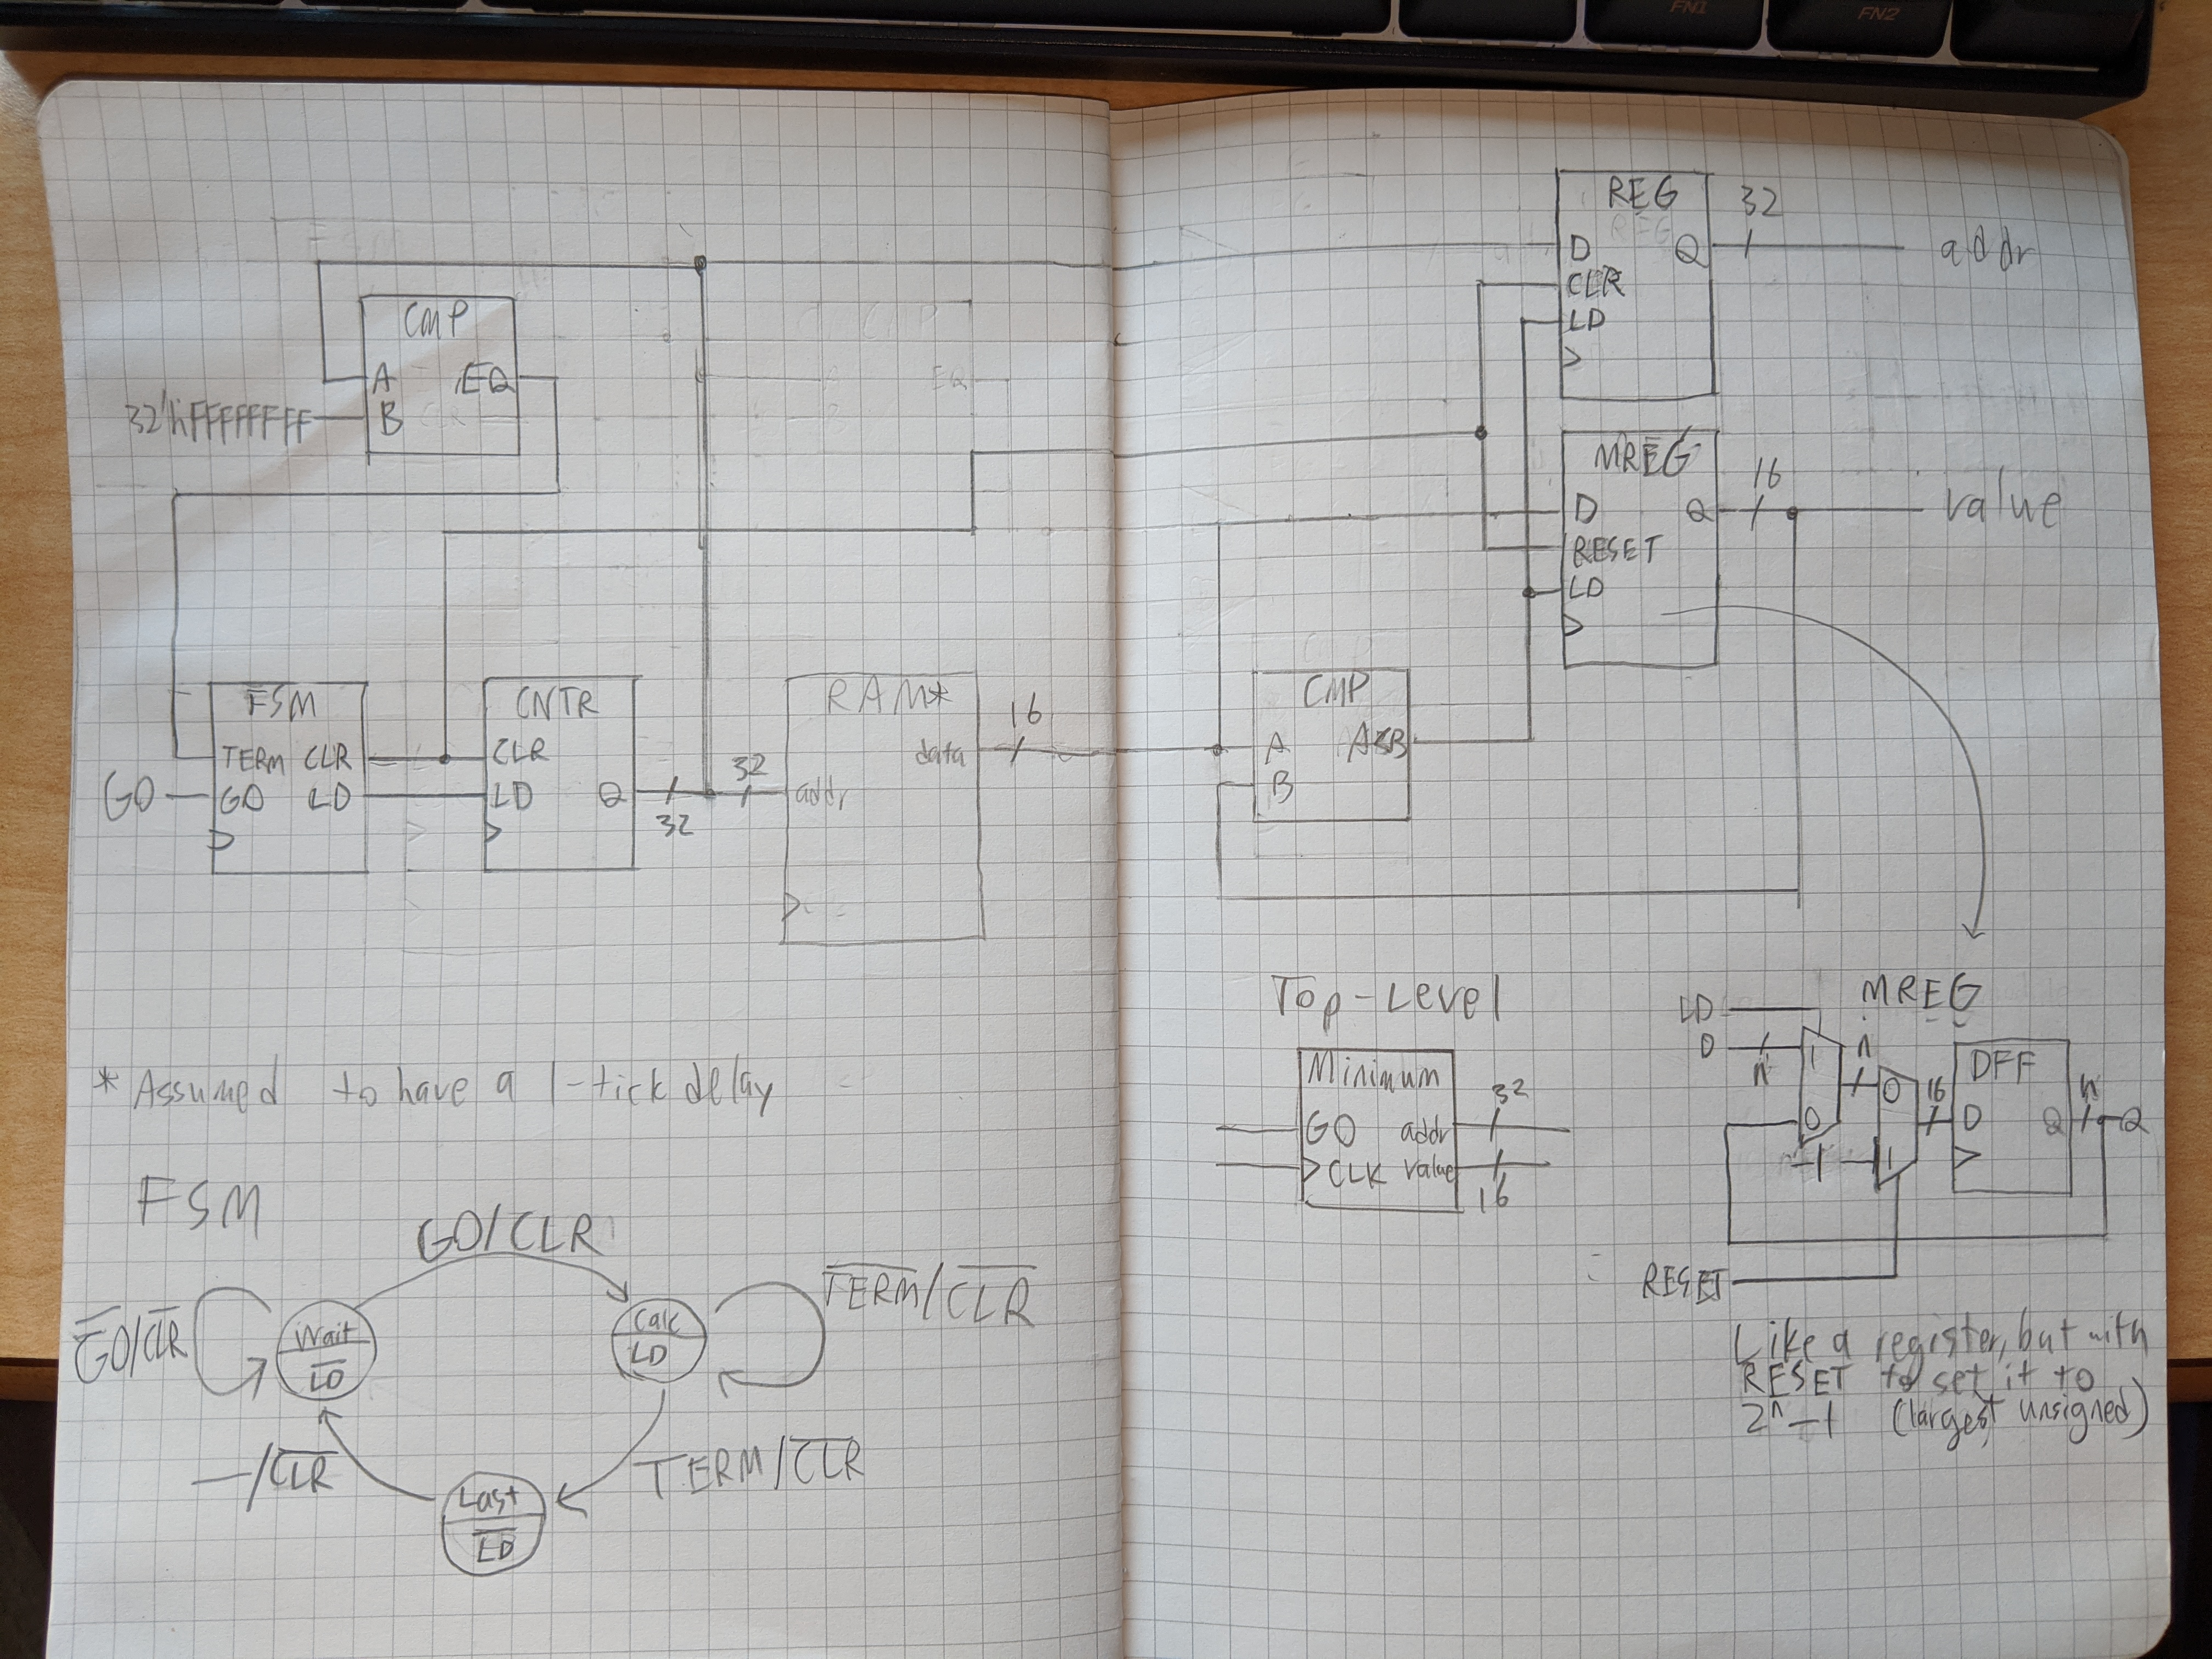
\includegraphics[width=\textwidth]{hw.jpg}
    
\end{document}